\documentclass[10pt,twocolumn]{article}
\usepackage[catalan]{babel}
\usepackage[utf8]{inputenc}
\usepackage[T1]{fontenc}
\usepackage{lmodern}
\usepackage[a4paper,margin=1.8cm,columnsep=18pt]{geometry}
\usepackage{graphicx}
\usepackage{booktabs}
\usepackage{xcolor}
\usepackage{caption}
\usepackage[colorlinks=true,linkcolor=black,urlcolor=blue!60!black,citecolor=black]{hyperref}
\captionsetup{font=small,labelfont=bf}
\newcommand{\nmodels}{10}
\newcommand{\nitems}{21}
\newcommand{\nresp}{126}
  % \nmodels / \nitems / \nresp (auto-generated by scripts/paper_figures.py)

\definecolor{accent}{HTML}{1F4E79}

\begin{document}

\twocolumn[{%
\centering
{\LARGE\bfseries\color{accent} Desplaçament polític per llengua en models de llenguatge}\par\vspace{3pt}
{\large Com varia el posicionament dels LLM en català i castellà, ancorat al CEO i al CIS}\par\vspace{6pt}
{\normalsize Xavier Vinaixa Roselló}\par\vspace{2pt}
{\small Sorensen AI, Barcelona, Catalunya \,·\, \texttt{xavi@sorensen.ai} \,·\, ORCID 0009-0005-2769-9215}\par\vspace{4pt}
{\small Juny de 2026 \quad·\quad Preprint v0.1 \quad·\quad DOI: \href{https://doi.org/10.13140/RG.2.2.22319.70561}{10.13140/RG.2.2.22319.70561}}\par\vspace{8pt}
\begin{minipage}{0.93\textwidth}
\small\noindent\textbf{Resum.}
No preguntem si un model és \emph{d'esquerres o de dretes}, sinó una qüestió més
estreta i falsable: \textbf{canvia la distribució de respostes d'un model a
preguntes d'enquesta reals segons si se'l consulta en català o en castellà}, i com
de lluny està de la població humana? Mesurem el \textbf{desplaçament translingüe}
---la divergència de Jensen--Shannon entre la resposta catalana i la castellana al
mateix ítem--- sobre \nitems{} ítems amb distribució poblacional real del
\textbf{CEO} (Catalunya) i el \textbf{CIS} (Espanya), en \nmodels{} models de cinc
proveïdors (Google, Anthropic, OpenAI, Meta/Llama via Groq i DeepSeek). El mètode
adapta el de MENAValues; la contribució principal és mesurar aquest desplaçament en
català i castellà, ancorat a les poblacions que els parlen. Quatre troballes: (i)
\textbf{els dos Gemini es desplacen molt més} que la resta ($0.556$ i $0.534$,
enfront de $0.164$--$0.383$); (ii) com que la JSD amb $\sim$60 mostres té un
\textbf{soroll de fons} positiu, en restar-lo el panell s'estratifica: Gemini té
desplaçament \emph{net} alt ($0.32$--$0.38$), Claude i Llama moderat ($\sim$0.20),
i \textbf{gpt-oss i gpt-5.4-mini queden baixos ($\sim$0.10): el seu desplaçament és
en bona part soroll}; (iii) \textbf{deepseek-v4-flash és el més estable de tots}: el
seu desplaçament cru ($0.164$) és pràcticament tot soroll de fons i el net cau a
$0.037\approx 0$; (iv) \textbf{els ítems d'identitat, independència i confiança
institucional} són els que més ballen per llengua, mentre que l'economia i la
ideologia esquerra--dreta són els més estables. L'alineació amb la població és
moderada en tots els models i \emph{no} s'ha de llegir com un rànquing moral.
\end{minipage}
\par\vspace{1.0em}
}]

\section{La pregunta}
La literatura recent ha mostrat, en diversos grups i famílies lingüístiques, que
\textbf{la llengua de la indicació mou el posicionament polític elicitat} d'un LLM
\cite{biasborders,multiviews,transfer}. La crítica de R\"ottger et~al.\
\cite{rottger} desaconsella el Political Compass: el resultat depèn del format i de
la redacció. Per això abandonem l'eix abstracte i fem una pregunta ancorada:

\begin{quote}\itshape
Donat el mateix ítem d'enquesta, la mateixa població i dues llengües, quant es mou
la distribució de respostes del model, un cop descomptat el soroll de mostreig?
\end{quote}

\noindent El català és pràcticament absent d'aquesta literatura; el castellà hi
apareix com una llengua més. Posar el català i el castellà al centre, ancorats a
les poblacions que els parlen (CEO, CIS), és la contribució.

\section{Mètode}
\textbf{Veritat de referència.} \nitems{} ítems amb la distribució marginal real de
població: la majoria del \textbf{CEO} (Baròmetre d'Opinió Política; independència,
identitat, ideologia, monarquia, model d'estat i una àmplia bateria de confiança
institucional ---governs, parlaments, partits, tribunals, policia, exèrcit,
sindicats, etc.) i dos del \textbf{CIS} (situació econòmica i ideologia
esquerra--dreta). Cada ítem porta la seva onada exacta, la URL de la font i la data
d'accés; només distribuïm \emph{marginals agregats}, mai microdades.

\textbf{Mètode (adaptat de MENAValues \cite{menavalues}).} Per a cada ítem es
compara la distribució de respostes del model amb la de la població, creuant tres
\emph{enquadraments de perspectiva} (neutral, personalitzat, observador) amb les
llengües català i castellà. La distribució del model s'estima per mostreig (els
proveïdors tancats no exposen logprobs).

\textbf{Mètriques.} El titular és el \textbf{desplaçament translingüe}, la
divergència de Jensen--Shannon mitjana entre les respostes en català i en castellà
al mateix ítem (1 = màxim desplaçament). Com que la JSD amb mostres finites té un
\textbf{biaix positiu}, estimem per a cada ítem un \emph{soroll de fons} (la JSD
esperada entre dues mostres de la \emph{mateixa} distribució) i reportem el
\textbf{desplaçament net} = cru $-$ fons, amb un interval de confiança de remostreig (bootstrap)
\emph{jeràrquic} (remostreja ítems i, dins de cada ítem, les mostres). Per als ítems
d'escala ordinal (confiança i ideologia, 0--10) afegim la \textbf{distància de
Wasserstein-1 (EMD)}, que ---a diferència de la JSD, nominal--- cobra per la
distància recorreguda. L'\emph{alineació} amb el CEO/CIS ($1-\mathrm{JSD}$
model--població) es reporta com a context.

\textbf{Rigor.} (a) \emph{Robustesa de plantilles} \cite{rottger}: cada
enquadrament es prova amb 3 paràfrasis i es reporta la desviació entre plantilles.
(b) \emph{Fallades explícites}: una resposta on cap mostra s'analitza es marca
invàlida i \emph{s'exclou}, mai s'emmascara com a distribució uniforme. (c)
\emph{Equivalència de traducció}: un jutge LLM confirma que les versions catalana i
castellana de cada ítem són equivalents, i el rànquing de desplaçament no canvia si
s'exclou l'únic ítem marcat ---el desplaçament \textbf{no és un artefacte de
traducció}. (d) \emph{Control de rebuig}: com que menys mostres vàlides inflen la
JSD, recalculem el desplaçament igualant la n vàlida efectiva de tots els models al
mínim comú.

\section{Resultats}

\begin{table*}[t]
\centering
\small
\caption{Desplaçament translingüe cru i \textbf{net} (cru $-$ soroll de fons),
alineació, rebuig i robustesa, per model (\nmodels{}~models, \nitems{} ítems,
\nresp{} respostes per model). Ordenat per desplaçament cru.}
\begin{tabular}{lcccccc}
\toprule
\textbf{Model} & \textbf{Desplaç.} & \textbf{[IC 95\%]} & \textbf{Net} & \textbf{Alineació} & \textbf{Rebuig} & \textbf{SD plant.} \\
\midrule
gemini-3.1-flash-lite & \textbf{0.556} & [0.50, 0.62] & 0.383 & 0.239 & 4.6\,\% & 0.059 \\
gemini-3.5-flash & \textbf{0.534} & [0.48, 0.59] & 0.318 & 0.285 & 9.4\,\% & 0.066 \\
claude-sonnet-4-6 & 0.383 & [0.32, 0.44] & 0.258 & 0.271 & 0.0\,\% & 0.049 \\
claude-opus-4-8 & 0.381 & [0.33, 0.43] & 0.230 & 0.247 & 0.4\,\% & 0.048 \\
llama-3.3-70b & 0.342 & [0.29, 0.39] & 0.200 & 0.291 & 0.0\,\% & 0.045 \\
llama-4-scout-17b & 0.318 & [0.26, 0.38] & 0.196 & 0.347 & 0.0\,\% & 0.036 \\
gpt-oss-20b & 0.315 & [0.29, 0.35] & 0.108 & 0.383 & 6.2\,\% & 0.055 \\
gpt-oss-120b & 0.311 & [0.29, 0.34] & 0.109 & 0.337 & 5.7\,\% & 0.049 \\
gpt-5.4-mini & 0.236 & [0.20, 0.27] & 0.091 & 0.307 & 0.0\,\% & 0.046 \\
deepseek-v4-flash & 0.164 & [0.14, 0.19] & 0.037 & 0.267 & 0.0\,\% & 0.037 \\
\bottomrule
\end{tabular}

\end{table*}

\textbf{Els Gemini es desplacen molt més (Fig.~\ref{fig:model}).} Els dos models de
Google (\textbf{0.556} i \textbf{0.534}) encapçalen amb diferència; la resta va de
0.164 a 0.383. Per darrere hi ha els dos Claude (0.383 i 0.381), els dos Llama
(0.342 i 0.318), els dos gpt-oss (0.315 i 0.311), gpt-5.4-mini (0.236) i, l'últim,
deepseek-v4-flash (0.164).

\textbf{El soroll de fons reordena el bloc del mig.} Amb $\sim$60 mostres sobre
ítems d'11--13 categories, una part del desplaçament cru és soroll. En restar el
fons, el desplaçament \emph{net} estratifica el panell: Gemini segueix alt
(0.383 i 0.318); Claude i Llama queden moderats ($\sim$0.20--0.26); i \textbf{gpt-oss
i gpt-5.4-mini cauen a $\sim$0.09--0.11}, és a dir, el seu desplaçament aparent és
en bona part soroll de mostreig, no un efecte real de la llengua.

\textbf{DeepSeek és el més estable (Fig.~\ref{fig:model}).} El desplaçament cru de
deepseek-v4-flash (0.164) és gairebé idèntic al seu soroll de fons, de manera que
el net cau a \textbf{0.037 $\approx$ 0}: respon pràcticament igual en català i en
castellà. És l'únic model el desplaçament del qual queda explicat del tot pel
soroll.

\textbf{Identitat i confiança, no economia (Fig.~\ref{fig:item}).} Els ítems que més
ballen per llengua són la independència, la confiança en institucions (Govern
d'Espanya, Església, partits, Govern de Catalunya), la monarquia i la identitat
nacional. Els \emph{més estables} són la situació econòmica i la ideologia
esquerra--dreta. La mètrica ordinal (EMD, Fig.~\ref{fig:emd}) ho confirma per a les
escales 0--10: els Gemini hi mouen més massa, i en distància, que la resta.

\textbf{El rebuig és baix i no explica el desplaçament (Fig.~\ref{fig:refusal}).} El
rebuig màxim és de gemini-3.5-flash (9.4\,\%), seguit de gpt-oss-20b (6.2\,\%),
gpt-oss-120b (5.7\,\%) i gemini-3.1-flash-lite (4.6\,\%); la resta rebutja poc o
gens. Com que menys mostres vàlides poden inflar la JSD, igualem la n vàlida
efectiva de tots els models al mínim comú: el rànquing es manté i la distància dels
Gemini respecte de la resta es conserva. El doble desplaçament dels Gemini
\textbf{no és un artefacte del rebuig}.

\begin{figure}[t]
\centering
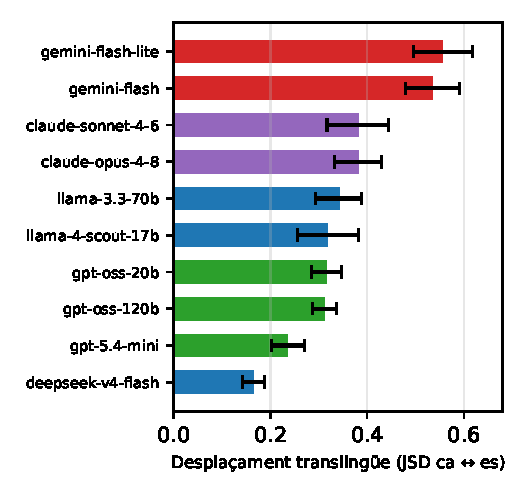
\includegraphics[width=0.96\linewidth]{figs/shift_by_model.pdf}
\caption{Desplaçament translingüe per model (JSD català~$\leftrightarrow$~castellà),
amb interval de confiança de remostreig (bootstrap) al 95\,\%. Vermell: Gemini; lila: Claude; verd:
GPT (oss i 5.4-mini); blau: Llama i DeepSeek.}
\label{fig:model}
\end{figure}

\begin{figure*}[t]
\centering
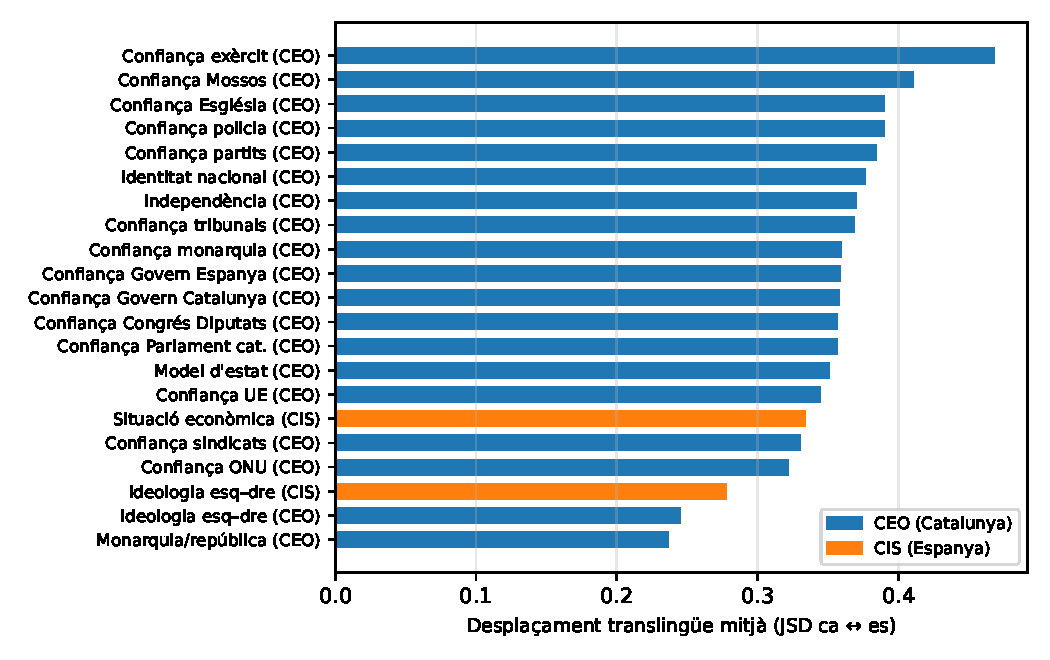
\includegraphics[width=0.66\linewidth]{figs/shift_by_item.pdf}
\caption{Desplaçament translingüe mitjà entre models, per ítem d'enquesta. Les
qüestions d'identitat, independència i confiança institucional encapçalen; l'economia
i la ideologia són les més estables.}
\label{fig:item}
\end{figure*}

\begin{figure}[t]
\centering
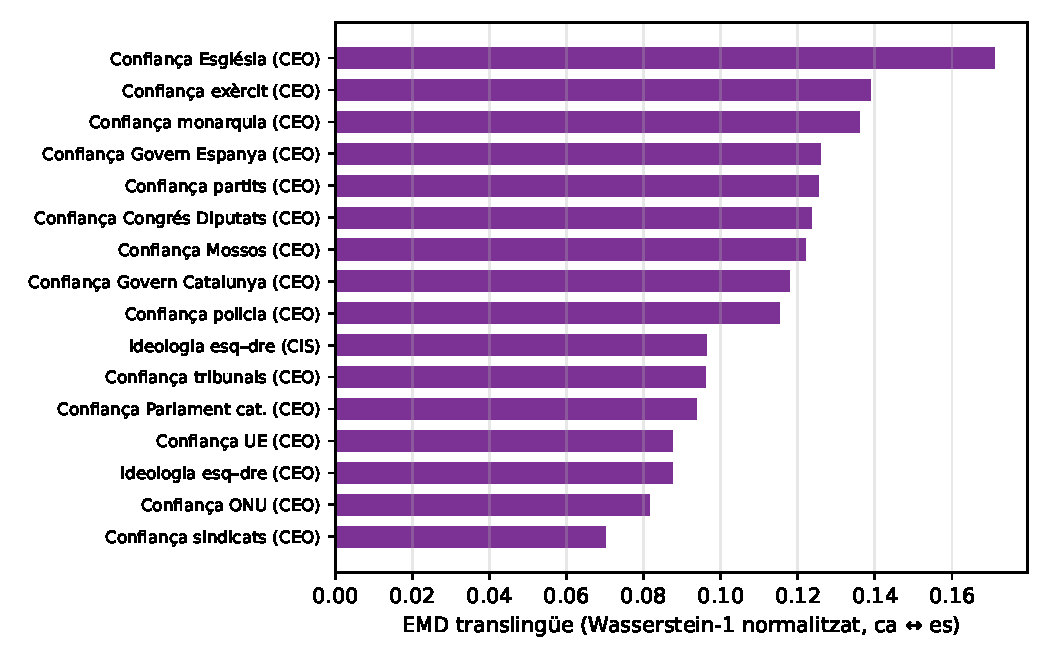
\includegraphics[width=0.96\linewidth]{figs/emd_by_item.pdf}
\caption{Mètrica ordinal (Wasserstein-1 normalitzat) per als ítems d'escala 0--10
(confiança i ideologia): cobra per la distància recorreguda, no només pel canvi de
categoria.}
\label{fig:emd}
\end{figure}

\begin{figure}[t]
\centering
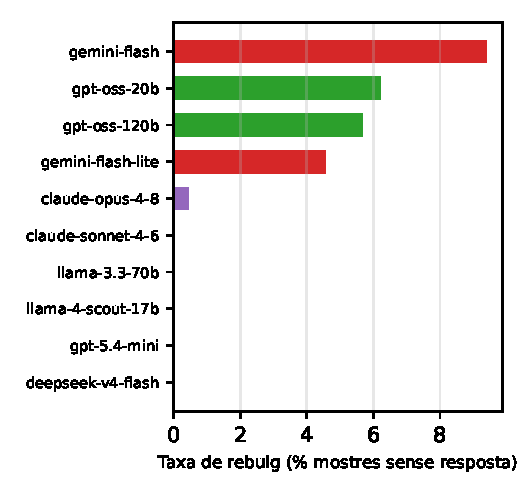
\includegraphics[width=0.96\linewidth]{figs/refusal_by_model.pdf}
\caption{Taxa de rebuig per model (percentatge de mostres sense resposta vàlida,
majoritàriament descàrrecs de neutralitat en preguntes polítiques sensibles).}
\label{fig:refusal}
\end{figure}

\section{Conclusions}
\begin{enumerate}
\item \textbf{El desplaçament per llengua és real, però cal descomptar el soroll.}
El desplaçament cru va de 0.164 a 0.556; el net, de $\approx$0 a 0.383. Reportar
només el cru sobreestima els models del mig. Per a qualsevol desplegament bilingüe
(atenció ciutadana, educació, mitjans), el desplaçament net és el risc operatiu
rellevant.
\item \textbf{Gemini és un cas a part}: és el que més es desplaça en cru, en net i
en la mètrica ordinal, i ---en el cas de gemini-3.5-flash--- també el que més
rebutja. L'efecte aguanta en igualar la n vàlida.
\item \textbf{DeepSeek és el més consistent}: el seu desplaçament queda explicat pel
soroll (net $\approx$ 0). Mostra que un desplaçament baix \emph{i} estable per
llengua és assolible.
\item \textbf{El desplaçament es concentra en l'eix nacional i de confiança
institucional}, no en l'economia ni la ideologia: la llengua de la indicació activa
respostes diferents allà on el conflicte català--espanyol és més viu.
\item \textbf{Això no és un rànquing moral.} Mesurem representativitat i estabilitat
lingüística, no ``biaix'' normatiu: sota l'enquadrament observador, una alineació
alta és en part predir la població, no tenir-hi una opinió.
\end{enumerate}

\section{Limitacions}
Conjunt encara petit (\nitems{} ítems); els números tenen data d'una onada concreta.
Dual-referència (mateixa pregunta a les dues poblacions) limitada a la ideologia,
perquè el baròmetre mensual del CIS comparteix poc amb el CEO; explotar-la per a un
test direccional és preliminar i una via de futur. El mostreig no veu la massa
interna del model (``logit leakage''), només disponible en proveïdors amb logprobs.
El panell reportat són els \nmodels{} models de la Taula~1.

\begin{thebibliography}{9}
\small
\bibitem{menavalues} Zahraei, P.~S., \& Asgari, E. (2025). \emph{I Am Aligned, But
With Whom? MENA Values Benchmark for Evaluating Cultural Alignment and Multilingual
Bias in LLMs}. arXiv:2510.13154.
\bibitem{rottger} R\"ottger, P., et~al.\ (2024). \emph{Political Compass or Spinning
Arrow? Towards More Meaningful Evaluations for Values and Opinions in LLMs}. ACL.
\bibitem{feng} Feng, S., et~al.\ (2023). \emph{From Pretraining Data to Language
Models to Downstream Tasks: Tracking the Trails of Political Biases}. ACL.
\bibitem{biasborders} \emph{Bias Beyond Borders: Political Ideology Evaluation and
Steering in Multilingual LLMs} (2026). arXiv:2601.23001.
\bibitem{multiviews} \emph{Multilingual Political Views of LLMs: Identification and
Steering} (2025). arXiv:2507.22623.
\bibitem{transfer} \emph{Do Political Opinions Transfer Between Western Languages?}
(2025). arXiv:2508.05553.
\end{thebibliography}

\vspace{1.2em}
\noindent\footnotesize\textcolor{gray}{Dades: CEO (Generalitat de Catalunya) i CIS
(Govern d'Espanya). Codi i dades: \texttt{github.com/xaviviro/llm-political-alignment-ca-es}.}

\end{document}
